\documentclass[a4paper,12pt]{article}
\usepackage[MeX]{polski}
\usepackage[utf8]{inputenc}
\usepackage{graphicx}
%opening
\title{Metro w Walencji}
\author{Bartłomiej Stando}

\begin{document}

\maketitle

\section{Metro w Walencji}
Metro w Walencji (hiszp. Valencia Metro) powstało na bazie wcześniejszej kolejki wąskotorowej. Pierwsza linia uruchomiona została w 1988 roku[1]. System dociera do odległych przedmieść. Długość wszystkich linii wynosi 134 kilometry z których tylko około 10% znajduje się pod ziemią. Część stacji została zaprojektowana przez Santiago Calatravę. Linia nr 4 jest zwykłą linią tramwajową po której kursuje 25 nowoczesnych tramwajów niskopodłogowych firmy Siemens. W roku 1996 Metro de Valencia przewiozło 20.040.483 pasażerów[2].
\begin{table}[here]
\begin{tabular}{|c|c|c|r|r|}
\hline
Linia & Trasa & Długość & Stacje & Pasażerowie w 2005\\
\hline
\hline
$1$ & Llíria – Villanueva de Castellón & 95.2 km & 58 & $19\,277\,123$\\
\hline
$3$ & Rafelbunyol – Aeroport & $19.8km$ & $21$ & $25\,450\,000$\\
\hline
$4$ & Mas del Rosari – Dr. Lluch & $9.8km$ & $32$ & $5\,088\,092$\\
\hline
$5$ & Neptú – Torrent Av ou Aeroport & $17.7km$ & $18$ & $11\,700\,000$\\
\hline
$6$ & Tossal del Rei – Marítim-Serrería	 & $10.8km$ & $22$ &  \\
\hline
\end{tabular}
\end{table}

\section {Galeria zdjęć}
\begin{figure}
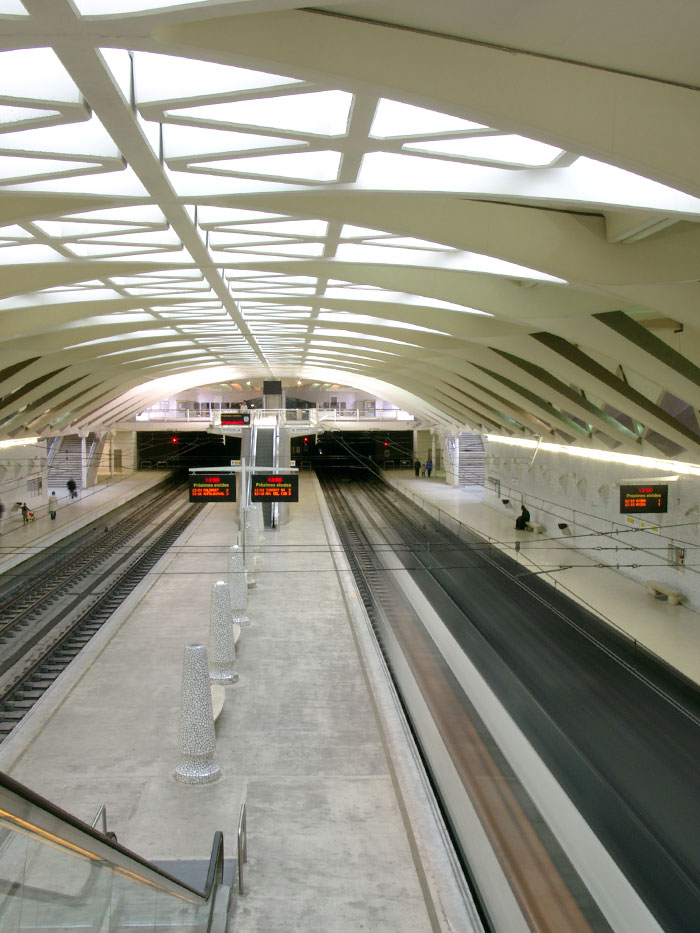
\includegraphics[width=0.15\hsize]{sta.jpg}
\caption{Stacja Alameda}\label{fig:Stacja Almeda}

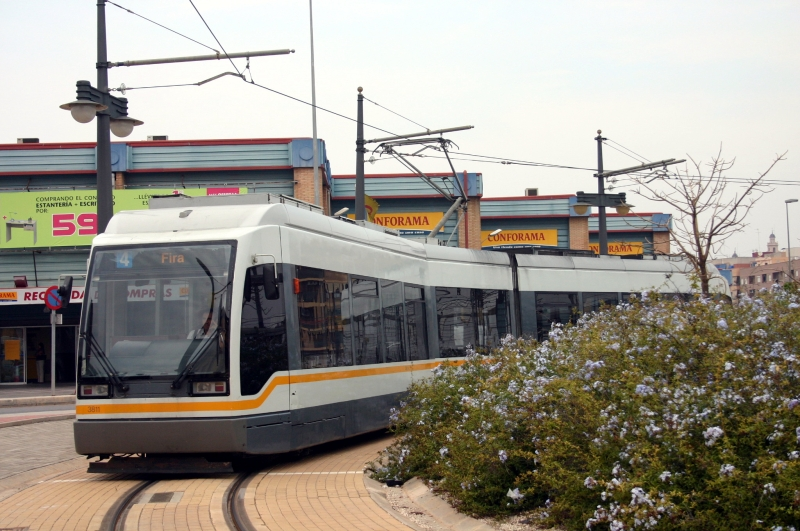
\includegraphics[width=0.15\hsize]{tramwaj.jpg}
\caption{Tramwaj typu CAF/Siemens na trasie linii T4}

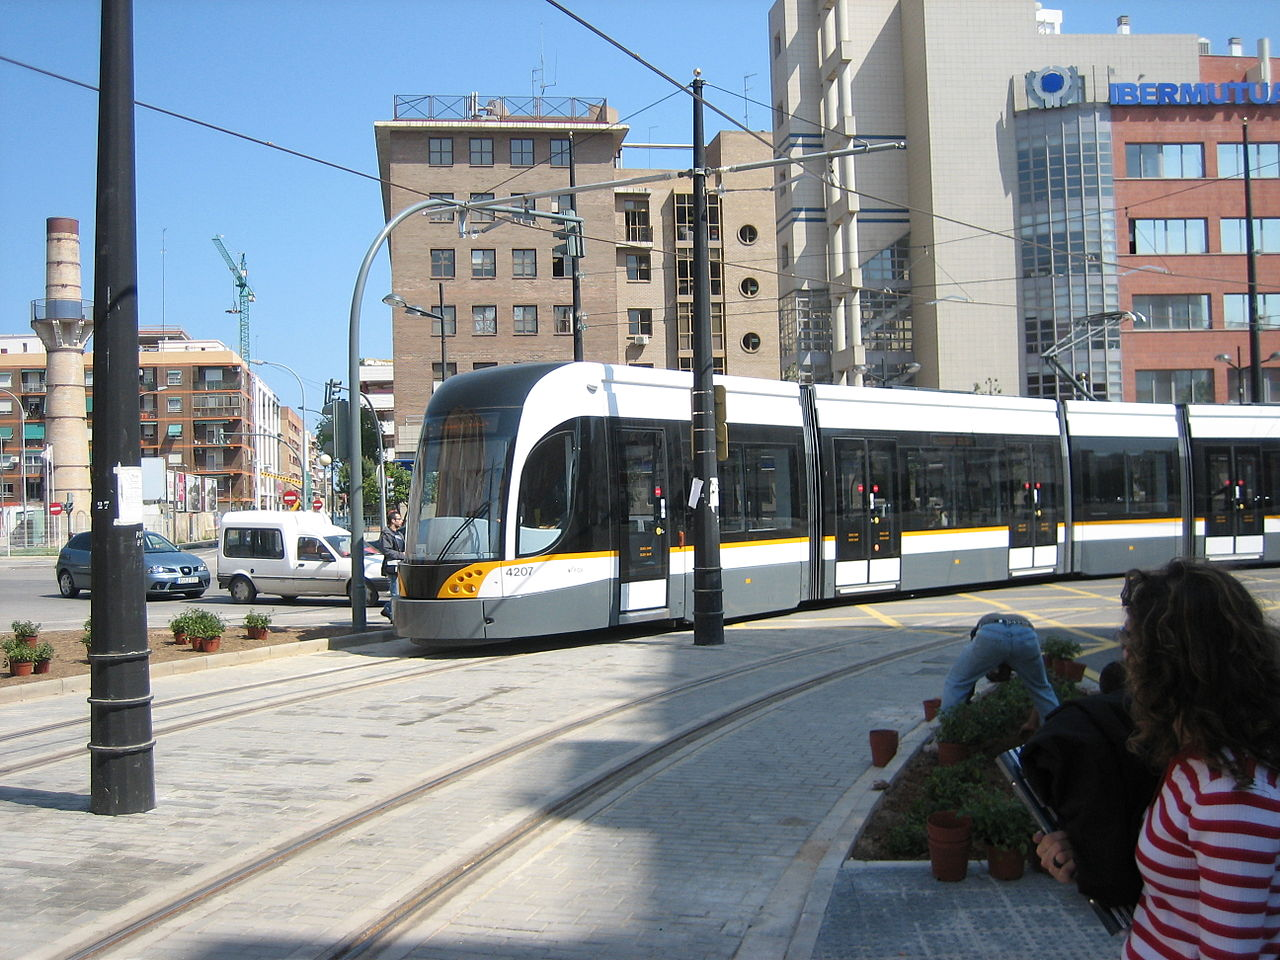
\includegraphics[width=0.15\hsize]{tramwaj2.jpg}
\caption{Tramwaj marki Bombardier Flexity Outlook Cityrunner}

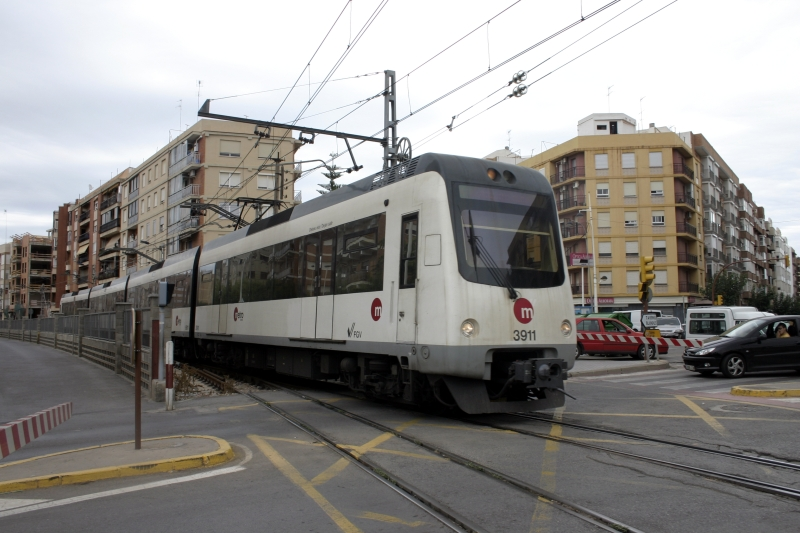
\includegraphics[width=0.15\hsize]{pociag.jpg}
\caption{Pociąg metra serii 3900}

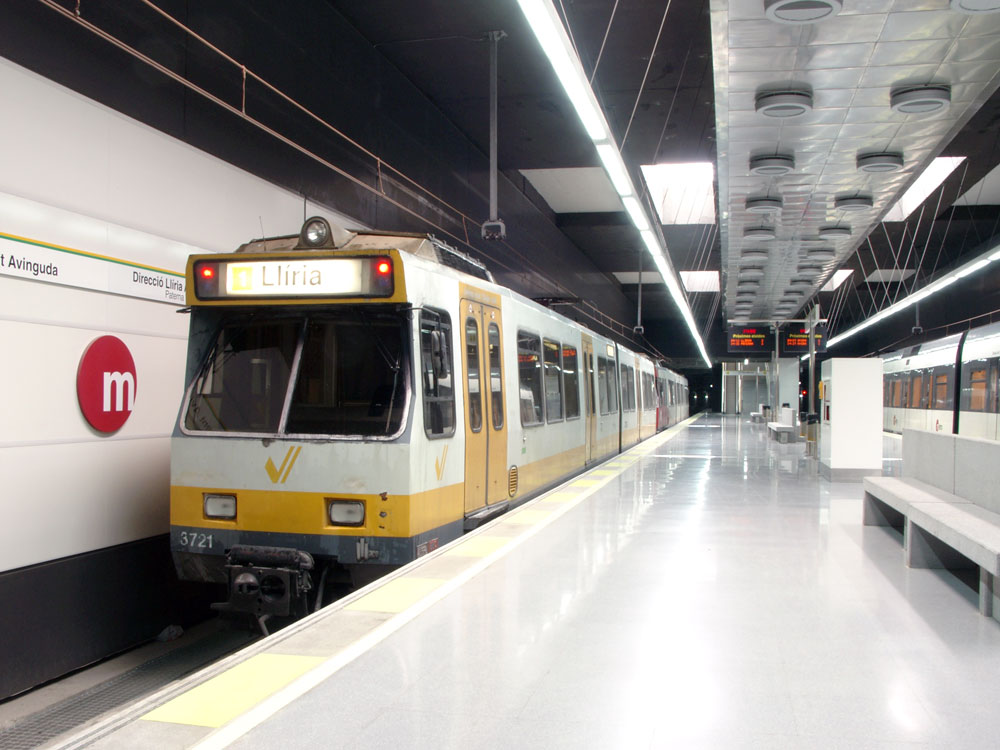
\includegraphics[width=0.15\hsize]{pociag2.jpg}
\caption{Pociąg serii 3700 na trasie linii 1 na stacji metra Torrent avinguda}

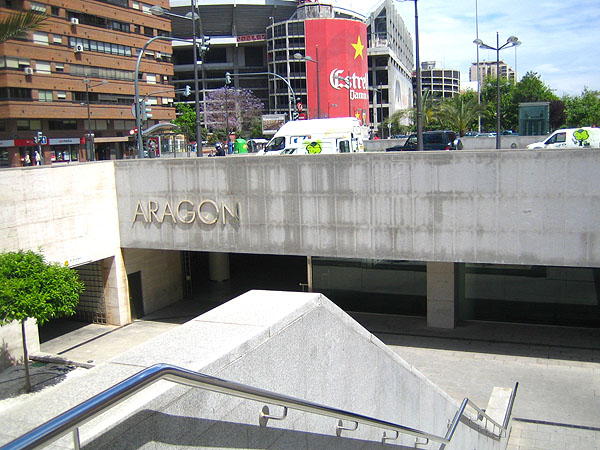
\includegraphics[width=0.15\hsize]{st.jpg}
\caption{Wejście do stacji metra Aragó}

\end{figure}

\section {Linki zewnetrzne}
\begin{itemize}
  \item Strona oficjalna
\item Informacje zdjęcia\ldots
\end{itemize}


\end{document}